%======================================================================
% U06a  第 6 章：假设检验的基本框架、两类错误、t 检验、把文字假设写成 Rβ = r
%======================================================================
\chapter{假设检验：t、F 与 Wald}
\label{ch:U06a-test}

第 5 章得到 $\sqrt n(\hat\beta-\beta)\dto N(0,V)$，且 $V$ 可以按同方差、HC、CRVE 三种方式一致地估计。本章把这两条结论变成\key{决策规则}：给定一个关于 $\beta$ 的假设，数据是否提供了足够的反对证据？路线是“一个约束 $\to$ 多个约束 $\to$ 一般框架”：先建立检验的语言（$H_0/H_1$、两类错误、size 与 power、临界值与 $p$ 值）；再讲单个约束的 t 检验，并把文字假设写成 $R\beta=r$；然后构造 Wald 统计量 $W\dto\chi^2_q$ 与两步 F 检验（$qF\dto\chi^2_q$，$t^2=W$）；最后讨论置信区间与检验的对偶、LM 与 LR 检验（拓展）、多重检验与 p-hacking。第 9 章的 IV/GMM 检验沿用本章的语言。对应 Hansen 第 9 章与 §7.13--§7.19。

%======================================================================
\section{假设检验的基本框架}\label{sec:U06a-frame}

%----------------------------------------------------------------------
\subsection{从估计到检验：\texorpdfstring{$\hat\beta=0.15$}{beta-hat = 0.15}，真值是 0 还是 1？}

\subsubsection{估计只给出一个数，真值仍然未知}

估计与检验回答的是不同的问题：
\[
\underbrace{\text{估计：}\ \hat\beta=0.15\ \longleftarrow\ \beta\ (?)}_{\text{用数据猜一个值}}
\qquad\Longrightarrow\qquad
\underbrace{\text{检验：}\ \beta=0\ \text{还是}\ \beta=1\,?}_{\text{判断某个具体的值是否可信}}
\]
OLS 给出一个数 $0.15$，但总体参数 $\beta$ 未知。检验问的是：某个事先给定的值（如 $0$ 或 $1$）与这个估计是否相容。

\subsubsection{用标准误衡量“距离”的大小}

$0.15$ 离 $0$ 有 $0.15$ 远，离 $1$ 有 $0.85$ 远。这些距离是“大”还是“小”，不能看绝对数值，要用 $\hat\beta$ 的抽样波动——\key{标准误}——来衡量：同样相差 $0.15$，标准误为 $0.01$ 时是 15 个标准误（远），标准误为 $0.5$ 时只有 0.3 个标准误（近）。假设检验就是把“距离”换算成“在 $H_0$ 下出现这么大距离的概率”：概率很小，就有理由怀疑 $H_0$。

%----------------------------------------------------------------------
\subsection{原假设与备择假设}

\subsubsection{定义：点假设 \texorpdfstring{$H_0:\theta=\theta_0$}{H0: theta = theta0} 与假设值}

设感兴趣的参数为 $\theta=r(\beta)\in\R^q$，$r(\cdot)$ 是 $\beta$（$K\times1$）的已知函数。例如 $\theta=\beta_j$（单个系数）、$\theta=\beta_j-\beta_l$（两系数之差）、$\theta=\beta_j/\beta_l$（两系数之比）。

\begin{defn}[原假设与备择假设]\label{def:U06a-hyp}
\begin{itemize}
  \item \term{原假设}{null hypothesis} $H_0:\theta=\theta_0$。$\theta_0$ 是研究者给定的已知数，称为\term{假设值}{hypothesized value}；单个系数的假设值常记作 $\beta_1^0$，即 $H_0:\beta_1=\beta_1^0$。这类“参数等于某一点”的假设称为\term{点假设}{point hypothesis}。
  \item \term{备择假设}{alternative hypothesis} $H_1$：$H_0$ 的补集，即参数空间中不满足 $H_0$ 的那些值。
\end{itemize}
（Hansen §9.1。）
\end{defn}

\subsubsection{双侧备择、单侧备择与联合假设的备择}

\begin{itemize}
  \item \term{双侧}{two-sided}备择：$H_1:\theta\ne\theta_0$。回归分析的默认选择。
  \item \term{单侧}{one-sided}备择：$H_1:\theta>\theta_0$ 或 $H_1:\theta<\theta_0$。何时可以用，见本章 t 检验一节。
  \item 多个约束（$q\ge2$）时，$H_1$ 写成“not $H_0$”：\key{至少一个}约束不成立，而不是“所有约束都不成立”。
\end{itemize}

\subsubsection{假设永远是关于总体参数的}

\begin{note}[假设的写法与结论的措辞]
\begin{itemize}
  \item 写 $H_0:\beta_1=0$，绝不能写 $H_0:\hat\beta_1=0$。$\hat\beta_1$ 是由数据算出的已知数，无需检验。
  \item 检验的结论只有两种：“拒绝 $H_0$”或“不拒绝 $H_0$”。“不拒绝”不等于“接受 $H_0$ 为真”，只表示证据不足（详见本章“多重检验、检验结果的误读与 p-hacking”一节）。英文写 “do not reject $H_0$”，少用 “accept $H_0$”。
\end{itemize}
\end{note}

%----------------------------------------------------------------------
\subsection{单个检验与联合检验：t、F、Wald 检验地图}

\subsubsection{单个假设与多重（联合）假设}

按约束个数区分两类假设：
\begin{enumerate}[label=(\alph*)]
  \item $H_0:\beta_1=\beta_1^0$：一个约束，称\term{单个检验}{single test}；
  \item $H_0:\beta_1=\beta_1^0$ 且 $\beta_2=\beta_2^0$：两个约束同时成立，称\term{多重检验}{multiple test} 或\term{联合检验}{joint test}。
\end{enumerate}
对应的检验统计量：(a) 用 \term{t 检验}{t-test}；(b) 用 \term{F 检验}{F-test}；(a) 与 (b) 都可以用 \term{Wald 检验}{Wald test}（又称 $\chi^2$ 检验）。F 检验也可以检验单个线性约束（此时 $F=t^2$），所以 F 检验与 Wald $\chi^2$ 检验都同时覆盖单个与多个约束。

\subsubsection{三种检验的适用范围与零分布}

\begin{center}
\small
\begin{tabularx}{\linewidth}{@{}l L l@{}}
\toprule
检验 & 适用的 $H_0$ & $H_0$ 下的（渐近）分布\\
\midrule
t 检验 & 一个约束（$q=1$），可做单侧或双侧 & $N(0,1)$（正态误差下精确为 $t_{n-K}$）\\
F 检验 & 一个或多个线性约束（同方差；两步法） & $F(q,\,n-K)$\\
Wald 检验 & 一个或多个约束，线性或非线性，可用稳健方差 & $\chi^2_q$\\
\bottomrule
\end{tabularx}
\captionof{table}{检验地图（$q$ 为约束个数，$K$ 为回归元个数）}
\end{center}
t 检验在本章 t 检验一节展开；Wald 检验、F 检验及二者的关系见本章后文。

\subsubsection{自由度由约束个数 \texorpdfstring{$q$}{q} 决定，而非涉及的系数个数}

\begin{note}[决定自由度的是“约束个数 $q$”]
$H_0:2\beta_1+3\beta_2=4$ 常被归入“多重检验”，因为它牵涉两个系数。但它只是\key{一个}线性约束（$q=1$），完全可以用 t 检验：
\[
t=\frac{2\hat\beta_1+3\hat\beta_2-4}{\mathrm{se}(2\hat\beta_1+3\hat\beta_2)},
\]
此时 $F=t^2$、$W=t^2$。而 $H_0:\beta_1=\beta_1^0$ 且 $\beta_2=\beta_2^0$ 是两个约束（$q=2$），必须用联合检验。
\end{note}

%----------------------------------------------------------------------
\subsection{显著性检验 \texorpdfstring{$H_0:\beta_1=0$}{H0: beta1 = 0} 与一般检验 \texorpdfstring{$H_0:\beta_1=1$}{H0: beta1 = 1}}

\subsubsection{显著性检验：\texorpdfstring{$x_1$}{x1} 对 \texorpdfstring{$y$}{y} 有没有影响}

\term{显著性检验}{significance test}是假设值为 0 的检验：
\[
H_0:\beta_1=0\qquad\text{vs}\qquad H_1:\beta_1\ne0 .
\]
它问的是“$x_1$ 对 $y$ 有没有影响”。Stata 回归表中每个系数旁的 \texttt{t} 与 \texttt{P>|t|} 都是这个检验。拒绝 $H_0$ 时称“$\beta_1$ \term{统计显著}{statistically significant}”。

\subsubsection{一般检验：单位弹性、购买力平价、CAPM}

假设值不必为 0。例如 $H_0:\beta_1=1$：单位弹性、购买力平价、CAPM 中 $\beta=1$ 等。做法与显著性检验相同，只需把 t 统计量的分子 $\hat\beta_1-0$ 换成 $\hat\beta_1-1$。

%----------------------------------------------------------------------
\subsection{检验统计量、接受域与拒绝域、临界值}

\begin{defn}[检验的构成]\label{def:U06a-test}
\begin{itemize}
  \item \term{检验统计量}{test statistic} $T=T(\text{data})$：数据的函数，设计成 $H_0$ 下倾向于取小值、$H_1$ 下倾向于取大值。最常用的是 t 统计量的绝对值 $T=|t|$。
  \item \term{临界值}{critical value} $c$：把样本空间分为\term{接受域}{acceptance region}（$T\le c$，不拒绝 $H_0$）与\term{拒绝域}{rejection region}（又称 critical region；$T>c$，拒绝 $H_0$）。
  \item \term{渐近零分布}{asymptotic null distribution}：$H_0$ 下 $T\dto\xi$，$\xi$ 的分布函数记为 $G(u)=P(\xi\le u)$。若 $G$ 不含未知参数，称 $T$ 是\term{渐近枢轴}{asymptotically pivotal}的。
\end{itemize}
\end{defn}

\subsubsection{检验统计量：\texorpdfstring{$H_0$}{H0} 下倾向于小、\texorpdfstring{$H_1$}{H1} 下倾向于大}

“$T$ 大”就是“数据与 $H_0$ 不相容”的证据。所以拒绝域总是取在 $T$ 的上尾。$|t|$、Wald 统计量 $W$、F 统计量都是按这一原则设计的非负统计量。

\subsubsection{临界值把样本空间分成接受域与拒绝域}

决策规则是
\[
\text{拒绝 }H_0\iff T>c,\qquad \text{不拒绝 }H_0\iff T\le c .
\]
$c$ 越大，拒绝越难。$c$ 怎样选，由下一节的 size 决定。

\subsubsection{渐近枢轴统计量的例子：\texorpdfstring{$|t|\dto|Z|$}{|t| -> |Z|} 与 \texorpdfstring{$W\dto\chi^2_q$}{W -> chi-square q}}

$H_0$ 下 $|t|\dto|Z|$（$Z\sim N(0,1)$），其分布函数为
\begin{align*}
G(u)=P(|Z|\le u)&=P(-u\le Z\le u) \why{绝对值不等式}\\
&=\Phi(u)-\Phi(-u) \why{$\Phi$ 为 $N(0,1)$ 分布函数}\\
&=\Phi(u)-[1-\Phi(u)]=2\Phi(u)-1, \why{对称性 $\Phi(-u)=1-\Phi(u)$}
\end{align*}
不含任何未知参数，所以 $|t|$ 渐近枢轴。同理 $W\dto\chi^2_q$ 也渐近枢轴。渐近枢轴的好处是：临界值可以直接从 $N(0,1)$ 或 $\chi^2_q$ 表中查出。

%----------------------------------------------------------------------
\subsection{检验的一般步骤}

\begin{method}[假设检验的七个步骤]
\begin{enumerate}
  \item 写出 $H_0$ 与 $H_1$（关于总体参数）；
  \item 选定显著性水平 $\alpha$（通常 5\%，也用 1\%、10\%）；
  \item 选检验统计量 $T$，写出它在 $H_0$ 下的（渐近）分布 $G$；
  \item 用数据算出 $T$ 的值（得到一个具体的数）；
  \item 求临界值 $c$（满足 $1-G(c)=\alpha$），或求 $p$ 值 $p=1-G(T)$；
  \item 决策：$T>c$（等价地 $p<\alpha$）则拒绝 $H_0$，否则不拒绝；
  \item 结合经济含义解释结论，并报告 $p$ 值与置信区间。
\end{enumerate}
\end{method}

\begin{english}
\textit{Template.} ``We test $H_0:\beta_1=0$ against $H_1:\beta_1\neq0$ at the 5\% significance level. Under $H_0$ the $t$-statistic $t=\hat\beta_1/\mathrm{se}(\hat\beta_1)$ is asymptotically $N(0,1)$. We reject $H_0$ if $|t|>1.96$, equivalently if the $p$-value is below 0.05.'' For joint hypotheses: ``The null hypothesis imposes $q=2$ linear restrictions, $H_0:R\beta=r$; the alternative is that at least one restriction fails.'' ``Failing to reject $H_0$ does not mean that $H_0$ is true; it only means that the evidence against it is insufficient.''
\end{english}

%======================================================================
\section{两类错误、size 与 power}\label{sec:U06a-errors}

检验根据随机的数据作决策，难免出错。本节先列出可能的错误，再定义衡量检验好坏的两个量：size（犯第一类错误的概率）与 power（$H_1$ 为真时拒绝 $H_0$ 的概率）。

%----------------------------------------------------------------------
\subsection{四种结局：第一类错误与第二类错误}

世界的真实状态有两种（$H_0$ 真或 $H_1$ 真），决策也有两种（拒绝或不拒绝 $H_0$），组合出四种结局：
\begin{center}
\begin{tabular}{@{}lcc@{}}
\toprule
 & 不拒绝 $H_0$ & 拒绝 $H_0$\\
\midrule
$H_0$ 为真 & 正确 & \textbf{第一类错误}（Type I error）\\
$H_1$ 为真 & \textbf{第二类错误}（Type II error） & 正确\\
\bottomrule
\end{tabular}
\captionof{table}{检验的四种结局（Hansen §9.5）}
\end{center}

\begin{defn}[两类错误]\label{def:U06a-errors}
\begin{itemize}
  \item \term{第一类错误}{Type I error}：$H_0$ 为真，却拒绝了它（“错杀”、虚假发现）。这是检验中被视为\key{严重}的错误。
  \item \term{第二类错误}{Type II error}：$H_1$ 为真（即 $H_0$ 是错的），却没有拒绝 $H_0$（“漏网”）。
\end{itemize}
\end{defn}

两类错误各有一个概率指标：
\[
\text{size}=P(\text{第一类错误})\ \ \text{（越小越好，常取 5\%、1\%）},\qquad
\text{power}=1-P(\text{第二类错误})\ \ \text{（越大越好）}.
\]
下面逐一定义。

%----------------------------------------------------------------------
\subsection{Size：控制第一类错误的概率}

\subsubsection{定义：size、渐近 size 与显著性水平}

\begin{defn}[size 与显著性水平]\label{def:U06a-size}
检验的\term{检验水平}{size}是犯第一类错误的概率：
\[
\text{size}=P(\text{reject }H_0\mid H_0\text{ true})=P(T>c\mid H_0).
\]
有限样本下这个概率通常算不出来，于是用\term{渐近水平}{asymptotic size}：
\[
\lim_{n\to\infty}P(T>c\mid H_0)=P(\xi>c)=1-G(c).
\]
研究者事先选定的上限 $\alpha$ 称为\term{显著性水平}{significance level}。
\end{defn}

\subsubsection{临界值的选取：\texorpdfstring{$1-G(c)=\alpha$}{1 - G(c) = alpha}}

给定 $\alpha$，取 $c$ 为 $G$ 的 $1-\alpha$ 分位数，即解 $1-G(c)=\alpha$，检验的渐近 size 就恰好等于 $\alpha$。这一步要求 $G$ 已知——这正是渐近枢轴统计量的方便之处。

\begin{exmp}[$|t|$ 检验取 $c=1.96$ 的渐近 size 为 5\%]
$H_0$ 下 $|t|\dto|Z|$，$Z\sim N(0,1)$。临界值 $c=1.96$ 时，
\solution
\begin{align*}
\lim_{n\to\infty}P(|t|>1.96\mid H_0)&=P(|Z|>1.96) \why{$|t|\dto|Z|$，1.96 是连续点}\\
&=P(Z>1.96)+P(Z<-1.96) \why{两个不相交事件}\\
&=[1-\Phi(1.96)]+\Phi(-1.96) \why{$\Phi$ 的定义}\\
&=2[1-\Phi(1.96)] \why{$\Phi(-a)=1-\Phi(a)$}\\
&=2(1-0.975)=0.05. \why{查表 $\Phi(1.96)=0.975$}
\end{align*}
一般地，$|t|$ 检验的渐近 size 为 $2[1-\Phi(c)]$。
\end{exmp}

%----------------------------------------------------------------------
\subsection{Power 与功效函数}

\begin{defn}[功效与功效函数]\label{def:U06a-power}
\term{功效}{power}是 $H_1$ 为真时拒绝 $H_0$ 的概率：
\[
\pi(\theta)=P(\text{reject }H_0\mid\theta)=1-P(\text{Type II error}),\qquad\theta\in H_1 .
\]
作为真值 $\theta$ 的函数，$\pi(\theta)$ 称为\term{功效函数}{power function}。
\end{defn}

功效依赖于真值 $\theta$ 与样本量 $n$。好的检验应当满足：$\theta$ 离 $\theta_0$ 越远、$n$ 越大，功效越高。在 $\theta=\theta_0$ 处，$\pi(\theta_0)$ 就是 size。

%----------------------------------------------------------------------
\subsection{病与没病的例子：为什么第一类错误更严重、如何选择 \texorpdfstring{$H_0$}{H0}}

\subsubsection{两种设定下的两类错误}

医生用一项检查判断病人是否患病。原假设有两种选法：
\begin{center}
\small
\begin{tabularx}{\linewidth}{@{}l L L@{}}
\toprule
 & 设定 1：$H_0$：有病（sick）\newline\phantom{设定 1：}$H_1$：没病 & 设定 2：$H_0$：没病（not sick）\newline\phantom{设定 2：}$H_1$：有病\\
\midrule
第一类错误 & \textbf{把病人判为健康} $\Rightarrow$ 不治疗，可能致命 & 把健康人判为有病 $\Rightarrow$ 多做检查、虚惊一场\\
第二类错误 & 把健康人判为有病 & \textbf{把病人判为健康}\\
被控制在 $\alpha$ 以内的错误 & 致命的错误（$\le5\%$） & 不太严重的错误；致命错误成了不受控制的第二类错误\\
\bottomrule
\end{tabularx}
\captionof{table}{病与没病：$H_0$ 的两种选法}
\end{center}

\subsubsection{原则：把“错误地拒绝它”代价最大的命题设为 \texorpdfstring{$H_0$}{H0}}

检验程序\key{只直接控制第一类错误的概率}（定为 $\alpha=5\%$ 甚至 1\%）；第二类错误的概率取决于未知的真值和样本量，常常很大且不受控制。因此：
\begin{itemize}
  \item 把“错误地拒绝它”代价最大的那个命题设为 $H_0$。这样最严重的错误就是第一类错误，被牢牢限制在 $\alpha$ 以内。这就是“第一类错误是严重错误”的含义。
  \item 医学筛查选设定 1，保护病人：只有证据很强时才判“没病”。
\end{itemize}

\subsubsection{法庭的无罪推定与实证研究中的“无效应”原假设}

\begin{itemize}
  \item 法庭上“无罪推定”：$H_0$ 为“无罪”，第一类错误是冤枉好人，被严格控制。
  \item 计量实证中，$H_0$ 通常取“无效应”（$\beta=0$）：在科学上，虚假地宣称发现了效应被视为更严重的错误；举证责任在主张“有效应”的研究者一方。
\end{itemize}

%----------------------------------------------------------------------
\subsection{Size 与 power 的权衡；“平凡功效”的检验}

\subsubsection{提高临界值：size 下降，power 也下降}

给定统计量 $T$，提高临界值 $c$：接受域变大、拒绝域变小 $\Rightarrow$ 第一类错误的概率（size）下降，但第二类错误的概率上升、power 下降。所以 $\alpha$ 不能任意小，否则检验失去功效。

\subsubsection{主流做法：在 size \texorpdfstring{$\le\alpha$}{<= alpha} 的约束下最大化 power}

检验设计的标准是：先保证 size 不超过 $\alpha$，再在满足这一约束的检验中选功效最高的（Hansen §9.5）。

\subsubsection{反例：随机拒绝的检验只有“平凡功效”}

\begin{note}[只看 size 是不够的]
考虑这样一个“检验”：抽一个与数据无关的 $U\sim U[0,1]$，若 $U<\alpha$ 则拒绝 $H_0$。它的 size 恰为 $P(U<\alpha)=\alpha$，但无论真值是什么，拒绝概率都是 $\alpha$，所以功效也恰为 $\alpha$。功效等于 size 的检验称为只有\term{平凡功效}{trivial power}，从中学不到任何东西。比较检验必须看功效。
\end{note}

%----------------------------------------------------------------------
\subsection{检验的一致性：\texorpdfstring{$n\to\infty$}{n -> infinity} 时 power \texorpdfstring{$\to1$}{-> 1}}

\subsubsection{例：正态均值检验的功效函数}

\begin{exmp}[正态均值检验的功效函数]\label{ex:U06a-power}
设 $y_1,\dots,y_n\overset{\iid}{\sim}N(\theta,\sigma^2)$，$\sigma$ 已知。检验 $H_0:\theta=0$ vs $H_1:\theta\ne0$，统计量 $T=\sqrt n\,\bar y/\sigma$，$|T|>1.96$ 时拒绝。求功效函数 $\pi(\theta)$。
\solution
先分解 $T$：加一项减一项 $\theta$，
\begin{align*}
T=\frac{\sqrt n\,\bar y}{\sigma}
&=\frac{\sqrt n(\bar y-\theta)}{\sigma}+\frac{\sqrt n\,\theta}{\sigma} \why{加一项减一项 $\theta$}\\
&=Z+\delta,\qquad Z\equiv\frac{\sqrt n(\bar y-\theta)}{\sigma}\sim N(0,1),\quad \delta\equiv\frac{\sqrt n\,\theta}{\sigma}. \why{$\bar y\sim N(\theta,\sigma^2/n)$}
\end{align*}
$\delta$ 是非随机的“漂移项”。于是
\begin{align*}
\pi(\theta)&=P(|Z+\delta|>1.96) \why{代入 $T$ 的分解}\\
&=P(Z+\delta>1.96)+P(Z+\delta<-1.96) \why{两侧拒绝域，不相交}\\
&=P(Z>1.96-\delta)+P(Z<-1.96-\delta) \why{移项}\\
&=[1-\Phi(1.96-\delta)]+\Phi(-1.96-\delta) \why{$\Phi$ 的定义}\\
&=\Phi\Bigl(\frac{\sqrt n\,\theta}{\sigma}-1.96\Bigr)+\Phi\Bigl(-\frac{\sqrt n\,\theta}{\sigma}-1.96\Bigr). \why{$1-\Phi(a)=\Phi(-a)$}
\end{align*}
三点含义：
\begin{itemize}
  \item $\theta=0$ 时 $\pi(0)=2\Phi(-1.96)=0.05$，正是 size。
  \item $\pi(\theta)$ 只通过 $\delta=\sqrt n\,\theta/\sigma$ 依赖于 $(\theta,n)$：$|\theta|$ 越大或 $n$ 越大，$|\delta|$ 越大，功效越高。样本量扩大 4 倍，同样功效所能识别的 $|\theta|$ 缩小一半（下表中 $n=25,\theta/\sigma=0.2$ 与 $n=100,\theta/\sigma=0.1$ 的功效都是 0.170）。
  \item 例如 $n=100$、$\theta/\sigma=0.1$：$\delta=1$，$\pi=\Phi(-0.96)+\Phi(-2.96)=0.1685+0.0015=0.170$。
\end{itemize}
\end{exmp}

\subsubsection{功效函数的数值与图形}

\begin{center}
\begin{minipage}[c]{0.40\linewidth}
\centering\small
\begin{tabular}{@{}cccc@{}}
\toprule
$\theta/\sigma$ & $n=25$ & $n=100$ & $n=400$\\
\midrule
0   & 0.050 & 0.050 & 0.050\\
0.1 & 0.079 & 0.170 & 0.516\\
0.2 & 0.170 & 0.516 & 0.979\\
0.3 & 0.323 & 0.851 & 1.000\\
0.4 & 0.516 & 0.979 & 1.000\\
\bottomrule
\end{tabular}
\captionof{table}{功效函数数值}
\end{minipage}\hfill
\begin{minipage}[c]{0.57\linewidth}
\centering
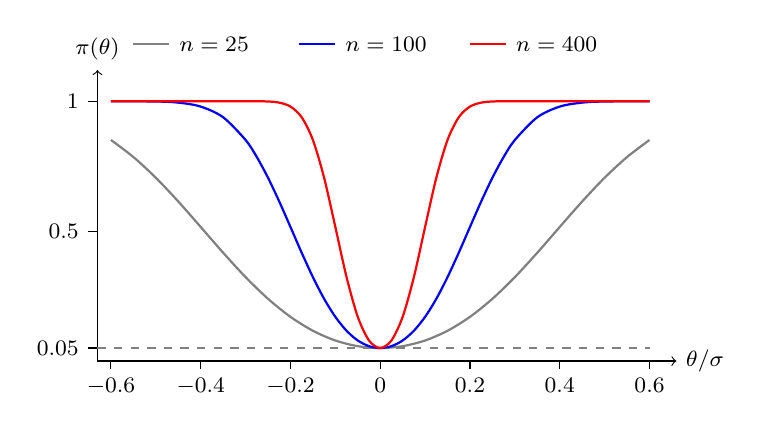
\begin{tikzpicture}[xscale=5.7,yscale=3.3,font=\footnotesize]
\draw[->] (-0.63,0) -- (0.66,0) node[right] {$\theta/\sigma$};
\draw[->] (-0.63,0) -- (-0.63,1.12) node[above] {$\pi(\theta)$};
\foreach \x in {-0.6,-0.4,-0.2,0,0.2,0.4,0.6} {\draw (\x,0) -- (\x,-0.03) node[below] {$\x$};}
\foreach \y in {0.5,1} {\draw (-0.63,\y) -- (-0.65,\y) node[left] {$\y$};}
\draw (-0.63,0.05) -- (-0.65,0.05) node[left] {$0.05$};
\draw[dashed,gray] (-0.63,0.05) -- (0.6,0.05);
\draw[thick,gray] plot[smooth] coordinates {(-0.600,0.8508) (-0.550,0.7852) (-0.500,0.7054) (-0.450,0.6141) (-0.400,0.5160) (-0.350,0.4169) (-0.300,0.3230) (-0.250,0.2395) (-0.200,0.1701) (-0.150,0.1165) (-0.100,0.0791) (-0.050,0.0572) (0.000,0.0500) (0.050,0.0572) (0.100,0.0791) (0.150,0.1165) (0.200,0.1701) (0.250,0.2395) (0.300,0.3230) (0.350,0.4169) (0.400,0.5160) (0.450,0.6141) (0.500,0.7054) (0.550,0.7852) (0.600,0.8508)};
\draw[thick,blue] plot[smooth] coordinates {(-0.600,1.0000) (-0.500,0.9988) (-0.450,0.9945) (-0.400,0.9793) (-0.350,0.9382) (-0.300,0.8508) (-0.275,0.7852) (-0.250,0.7054) (-0.225,0.6141) (-0.200,0.5160) (-0.175,0.4169) (-0.150,0.3230) (-0.125,0.2395) (-0.100,0.1701) (-0.075,0.1165) (-0.050,0.0791) (-0.025,0.0572) (0.000,0.0500) (0.025,0.0572) (0.050,0.0791) (0.075,0.1165) (0.100,0.1701) (0.125,0.2395) (0.150,0.3230) (0.175,0.4169) (0.200,0.5160) (0.225,0.6141) (0.250,0.7054) (0.275,0.7852) (0.300,0.8508) (0.350,0.9382) (0.400,0.9793) (0.450,0.9945) (0.500,0.9988) (0.600,1.0000)};
\draw[thick,red] plot[smooth] coordinates {(-0.600,1.0000) (-0.300,1.0000) (-0.250,0.9988) (-0.225,0.9945) (-0.200,0.9793) (-0.175,0.9382) (-0.150,0.8508) (-0.125,0.7054) (-0.100,0.5160) (-0.075,0.3230) (-0.050,0.1701) (-0.025,0.0791) (0.000,0.0500) (0.025,0.0791) (0.050,0.1701) (0.075,0.3230) (0.100,0.5160) (0.125,0.7054) (0.150,0.8508) (0.175,0.9382) (0.200,0.9793) (0.225,0.9945) (0.250,0.9988) (0.300,1.0000) (0.600,1.0000)};
\draw[thick,gray] (-0.55,1.22) -- (-0.47,1.22) node[right,black] {$n=25$};
\draw[thick,blue] (-0.18,1.22) -- (-0.10,1.22) node[right,black] {$n=100$};
\draw[thick,red] (0.20,1.22) -- (0.28,1.22) node[right,black] {$n=400$};
\end{tikzpicture}
\captionof{figure}{功效函数（$\theta=0$ 处等于 size 0.05）}
\end{minipage}
\end{center}

图中三条曲线都在 $\theta=0$ 处取最小值 0.05，向两侧单调上升；$n$ 越大，曲线越陡，越快升到 1。

\subsubsection{一致检验的定义；t 检验与 Wald 检验都是一致的}

\begin{thm}[检验的一致性]\label{thm:U06a-consistent}
若对任意固定的 $\theta\in H_1$，$\lim_{n\to\infty}\pi(\theta)=1$，则称该检验为\term{一致检验}{consistent test}。在第 5 章的假设下，t 检验与 Wald 检验都是一致检验（Hansen §9.21）。
\end{thm}

以 t 检验为例说明原因。设 $\sqrt n(\hat\theta-\theta)\dto N(0,V_\theta)$，$\hat V_\theta\pto V_\theta>0$，真值 $\theta\ne\theta_0$ 固定。把 t 统计量分解为
\begin{align*}
t=\frac{\sqrt n(\hat\theta-\theta_0)}{\sqrt{\hat V_\theta}}
&=\frac{\sqrt n(\hat\theta-\theta)}{\sqrt{\hat V_\theta}}+\frac{\sqrt n(\theta-\theta_0)}{\sqrt{\hat V_\theta}} \why{加一项减一项 $\theta$}\\
&=\underbrace{\frac{\sqrt n(\hat\theta-\theta)}{\sqrt{\hat V_\theta}}}_{\dto N(0,1)}
+\underbrace{\sqrt n\cdot\frac{\theta-\theta_0}{\sqrt{\hat V_\theta}}}_{\text{绝对值以 }\sqrt n\text{ 速度发散}} . \why{Slutsky；系数 $\pto$ 非零常数}
\end{align*}
第一项依概率有界，第二项的绝对值趋于无穷，所以对任何固定的临界值 $c$，$P(|t|>c)\to1$。Wald 统计量同理：$H_1$ 下 $W=n(R\hat\beta-r)\T(R\hat VR\T)\inv(R\hat\beta-r)$ 中 $R\hat\beta-r\pto R\beta-r\ne0$，$W$ 以 $n$ 的速度发散。

\subsubsection{推论：样本足够大时，任何固定偏离都会被拒绝}

一致性的另一面：样本足够大时，与 $\theta_0$ 的\key{任何}固定偏离——哪怕经济上微不足道——都会被拒绝。这就是“样本足够大，什么假设都会被拒绝”的含义（Hansen 练习 9.13）：点假设几乎不会严格成立，大样本下“统计显著”几乎必然出现，所以必须同时看效应大小（见本章 t 检验一节“统计显著与经济显著”，以及本章“多重检验、检验结果的误读与 p-hacking”一节）。

%----------------------------------------------------------------------
\subsection{练习：size 相同的检验未必同样好}

\begin{prac}[一个“奇怪”的检验（改编自 Hansen 练习 9.3）]
检验 $H_0:\theta=0$ vs $H_1:\theta\ne0$，$H_0$ 下 $|T|\dto|Z|$，$Z\sim N(0,1)$。有人提议：当 $|T|<c_1$ 或 $|T|>c_2$ 时拒绝，其中 $c_1$、$c_2$ 分别是 $|Z|$ 的 $\alpha/2$ 与 $1-\alpha/2$ 分位数。(a) 证明其渐近 size 为 $\alpha$。(b) 这是好检验吗？
\answer
(a) 由分位数的定义，$P(|Z|\le c_1)=\alpha/2$，$P(|Z|\le c_2)=1-\alpha/2$；$c_1<c_2$，两个拒绝事件不相交。$H_0$ 下
\begin{align*}
P(\text{reject}\mid H_0)&=P(|T|<c_1)+P(|T|>c_2) \why{两事件不相交}\\
&\to P(|Z|<c_1)+P(|Z|>c_2) \why{$|T|\dto|Z|$，$|Z|$ 连续}\\
&=\frac\alpha2+\Bigl[1-\Bigl(1-\frac\alpha2\Bigr)\Bigr] \why{分位数的定义}\\
&=\alpha .
\end{align*}
$\alpha=5\%$ 时，由 $P(|Z|\le c)=2\Phi(c)-1$ 得 $c_1=\Phi\inv(0.5125)\approx0.031$，$c_2=\Phi\inv(0.9875)\approx2.241$。

(b) 不好。理由有三：
\begin{itemize}
  \item 它在 $|T|$ 很小——即估计值最接近 $H_0$——时拒绝 $H_0$，违背“$T$ 大才是反对 $H_0$ 的证据”的检验逻辑。
  \item 拒绝概率中有 $\alpha/2$ 被“浪费”在最支持 $H_0$ 的区域，上侧临界值只好从 1.96 提高到 2.241。在备择 $T\approx Z+\delta$ 下，$|Z+\delta|<0.031$ 的概率极小，于是它的功效对每一个备择都低于标准检验 $|T|>z_{1-\alpha/2}$。数值计算：$\alpha=5\%$ 时最多低约 11 个百分点（$\delta\approx2.15$ 处，0.465 对 0.575）；功效仍不低于 $\alpha$。
  \item 结论：size 相同不代表检验同样好，必须比较功效。Wald 版本——$W<c_1$ 或 $W>c_2$ 时拒绝（Hansen 练习 9.4）——同理不可取：$W$ 小是支持 $H_0$ 的证据。
\end{itemize}
\end{prac}

\begin{english}
\textit{Template.} ``A Type I error occurs when a true null is rejected; its probability is the size of the test, which we control at $\alpha=5\%$. A Type II error occurs when a false null is not rejected; the power of the test is one minus its probability. Since only the Type I error probability is controlled, the hypothesis whose false rejection is most costly should be taken as the null. The test is consistent: for any fixed alternative its power tends to one as $n\to\infty$. Hence in very large samples even economically negligible deviations from $H_0$ will be detected.''
\end{english}

%======================================================================
\section{t 检验}\label{sec:U06a-t}

本节处理\key{单个约束}：$H_0:\theta=\theta_0$，其中 $\theta=r(\beta)\in\R$ 是一个实数参数（单个系数 $\beta_1$，或线性组合 $2\beta_1+3\beta_2$，或非线性函数 $\beta_1/\beta_2$）。

%----------------------------------------------------------------------
\subsection{t 统计量及其渐近零分布}

\subsubsection{t 统计量的定义与记号 \texorpdfstring{$\overset{a}{\sim}$}{(asymptotically distributed)}}

检验 $H_0:\beta_1=\beta_1^0$ vs $H_1:\beta_1\ne\beta_1^0$ 的 \term{t 统计量}{t-statistic}为
\begin{equation}\label{eq:U06a-t}
t_1=\frac{\hat\beta_1-\beta_1^0}{\mathrm{se}(\hat\beta_1)}\ \overset{a}{\sim}\ N(0,1)\qquad\text{under }H_0 ,
\end{equation}
分子是估计值与假设值之差，分母是估计值的标准误。$\beta_1^0=0$ 时就是显著性检验，$t_1=\hat\beta_1/\mathrm{se}(\hat\beta_1)$，常称 t-ratio。记号 $\overset{a}{\sim}$ 读作“\term{渐近服从}{asymptotically distributed}”，即样本量趋于无穷时的极限分布；\eqref{eq:U06a-t} 说 $t_1$ \term{渐近正态}{asymptotically normal}。

决策时，把 $\hat\beta_1$、$\beta_1^0$、$\mathrm{se}(\hat\beta_1)$ 代入，$t_1$ 就成为一个具体的数，再把这个数放到 $N(0,1)$ 分布中看它是否“极端”：$|t_1|>1.96$ 在 5\% 水平拒绝，$|t_1|>2.58$ 在 1\% 水平拒绝。

\subsubsection{定理：\texorpdfstring{$H_0$}{H0} 下 \texorpdfstring{$t\dto N(0,1)$}{t -> N(0,1)}}

\begin{thm}[t 检验的渐近零分布]\label{thm:U06a-t}
在第 5 章的假设下，设 $\theta=r(\beta)\in\R$，$\hat\theta=r(\hat\beta)$，$H_0:\theta=\theta_0$ 成立，则
\[
t=\frac{\hat\theta-\theta_0}{\mathrm{se}(\hat\theta)}\ \dto\ N(0,1).
\]
取 $c$ 满足 $\alpha=2[1-\Phi(c)]$，则检验“$|t|>c$ 时拒绝 $H_0$”的渐近 size 为 $\alpha$（Hansen §9.4）。
\end{thm}

\subsubsection{推导：分子用渐近正态，分母用一致性，合成用 Slutsky}

记号：$\sqrt n(\hat\theta-\theta)\dto N(0,V_\theta)$，$V_\theta>0$。线性情形 $\theta=R\beta$（$R$ 为 $1\times K$）时 $V_\theta=RVR\T$；非线性情形由 Delta 方法，$V_\theta=RVR\T$，$R=\partial r(\beta)/\partial\beta\T$（第 5 章）。$\hat V_\theta\pto V_\theta$ 是其一致估计，$\mathrm{se}(\hat\theta)=\sqrt{\hat V_\theta/n}$。要证 $H_0$ 下 $t\dto N(0,1)$：
\begin{align*}
t=\frac{\hat\theta-\theta_0}{\mathrm{se}(\hat\theta)}
&=\frac{\hat\theta-\theta_0}{\sqrt{\hat V_\theta/n}} \why{se 的定义}\\
&=\frac{\sqrt n(\hat\theta-\theta_0)}{\sqrt{\hat V_\theta}} \why{分子分母同乘 $\sqrt n$}\\
&=\frac{\sqrt n(\hat\theta-\theta)}{\sqrt{\hat V_\theta}} \why{$H_0$：$\theta=\theta_0$}\\
\sqrt n(\hat\theta-\theta)&\dto \xi\sim N(0,V_\theta) \why{第 5 章渐近正态（或 Delta 方法）}\\
\sqrt{\hat V_\theta}&\pto\sqrt{V_\theta}>0 \why{CMT：$\sqrt{\cdot}$ 连续}\\
t&\dto \frac{\xi}{\sqrt{V_\theta}} \why{Slutsky 定理}\\
\frac{\xi}{\sqrt{V_\theta}}&\sim N\Bigl(0,\frac{V_\theta}{V_\theta}\Bigr)=N(0,1). \why{$\Var(a\xi)=a^2\Var(\xi)$}
\end{align*}
由此 $|t|\dto|Z|$，$P(|t|>c\mid H_0)\to P(|Z|>c)=2[1-\Phi(c)]=\alpha$。这说明 t 统计量渐近枢轴：临界值只需查 $N(0,1)$ 表。

\subsubsection{标准误必须与误差结构匹配：同方差、HC、CRVE}

上面推导的关键是 $\hat V_\theta\pto V_\theta$，即 se 用的方差公式必须与误差结构一致：同方差时用同方差公式，独立异方差时用 HC（White）公式，组内相关时用 CRVE（第 5 章）。若用错——如异方差或聚类时仍用同方差 se——分母不再收敛到正确的值，$t$ 的极限不是 $N(0,1)$，检验的真实 size 偏离名义水平（通常过度拒绝）。

%----------------------------------------------------------------------
\subsection{双侧检验的临界值：1.645、1.96、2.58}

\subsubsection{由 \texorpdfstring{$\alpha=2[1-\Phi(c)]$}{alpha = 2[1 - Phi(c)]} 解出 \texorpdfstring{$c=z_{1-\alpha/2}$}{c = z(1-alpha/2)}}

记 $z_\tau=\Phi\inv(\tau)$ 为 $N(0,1)$ 的 $\tau$ 分位数。双侧检验的临界值由 size 条件解出：
\begin{align*}
\alpha=2[1-\Phi(c)]
&\iff \Phi(c)=1-\frac\alpha2 \why{移项}\\
&\iff c=\Phi\inv\Bigl(1-\frac\alpha2\Bigr)\equiv z_{1-\alpha/2}. \why{$\Phi$ 严格递增}
\end{align*}
例如 $\alpha=5\%$：$c=z_{0.975}=1.96$。单侧检验把全部 $\alpha$ 放在一侧，临界值为 $z_{1-\alpha}$（见下一小节）。

\subsubsection{临界值表与星号惯例}

\begin{center}
\begin{tabular}{@{}cccc@{}}
\toprule
显著性水平 $\alpha$ & 双侧临界值 $z_{1-\alpha/2}$ & 单侧临界值 $z_{1-\alpha}$ & 星号惯例\\
\midrule
10\% & 1.645 & 1.282 & *\\
5\% & 1.960 & 1.645 & **\\
1\% & 2.576（$\approx2.58$） & 2.326 & ***\\
\bottomrule
\end{tabular}
\captionof{table}{标准正态临界值}
\end{center}
星号惯例：$|t|$ 超过 10\%、5\%、1\% 的双侧临界值，分别标 *、**、***。

\subsubsection{常用标准正态分布函数值}

开卷考试可直接查下表（$\Phi(-z)=1-\Phi(z)$；最后一行是双侧 $p$ 值 $2[1-\Phi(z)]$）：
\begin{center}
\footnotesize
\setlength{\tabcolsep}{3.6pt}
\begin{tabular}{@{}l*{12}{c}@{}}
\toprule
$z$ & 0.5 & 0.8 & 1.0 & 1.5 & 1.645 & 1.7 & 1.96 & 2.0 & 2.2 & 2.5 & 2.576 & 3.0\\
\midrule
$\Phi(z)$ & .6915 & .7881 & .8413 & .9332 & .9500 & .9554 & .9750 & .9772 & .9861 & .9938 & .9950 & .9987\\
$2[1-\Phi(z)]$ & .617 & .424 & .317 & .134 & .100 & .089 & .050 & .046 & .028 & .012 & .010 & .003\\
\bottomrule
\end{tabular}
\captionof{table}{常用 $\Phi$ 值与双侧 $p$ 值}
\end{center}

%----------------------------------------------------------------------
\subsection{单侧检验（1.645）与何时使用}

\subsubsection{单侧检验的拒绝规则与单侧 \texorpdfstring{$p$}{p} 值}

单侧检验用\key{带符号}的 t 统计量 $t=(\hat\theta-\theta_0)/\mathrm{se}(\hat\theta)$：
\begin{itemize}
  \item $H_0:\theta=\theta_0$ vs $H_1:\theta>\theta_0$：$t>z_{1-\alpha}$ 时拒绝；5\% 水平即 $t>1.645$。负的 $t$ 不构成支持 $\theta>\theta_0$ 的证据。单侧 $p$ 值为 $p=1-\Phi(t)$。
  \item $H_0:\theta=\theta_0$ vs $H_1:\theta<\theta_0$：$t<-z_{1-\alpha}$ 时拒绝；5\% 水平即 $t<-1.645$。单侧 $p$ 值为 $p=\Phi(t)$。
\end{itemize}
临界值的来源：$H_0$ 下 $P(t>c)\to1-\Phi(c)$，令其等于 $\alpha$，得 $c=z_{1-\alpha}$。单侧临界值小于双侧临界值，所以同一个 $t$ 更容易在单侧检验中被拒绝。

\subsubsection{何时用单侧检验：参数空间事先只能在一侧}

只有当参数空间事先已知只能在一侧（如经济理论保证 $\theta\ge\theta_0$）时，单侧检验才合理。回归系数通常没有先验的符号限制，所以惯例用\key{双侧}检验（Hansen §9.4）。统计学教科书偏重单侧检验，主要是因为它在理论上更简洁。

%----------------------------------------------------------------------
\subsection{决策规则一：临界值法}

\begin{method}[临界值法]
\begin{itemize}
  \item t 检验：$|t|>$ 临界值 $\Rightarrow$ 拒绝 $H_0$；否则不拒绝。
  \item 同一逻辑适用于 F 与 Wald 检验：$F>$ 临界值（或 $W>$ 临界值）$\Rightarrow$ 拒绝 $H_0$。
\end{itemize}
\end{method}

\begin{center}
\begin{tikzpicture}[xscale=1.3,yscale=7,font=\scriptsize]
\fill[cthm!25] (1.96,0) -- plot[domain=1.96:3.6,samples=40] (\x,{0.3989*exp(-\x*\x/2)}) -- (3.6,0) -- cycle;
\fill[cthm!25] (-3.6,0) -- plot[domain=-3.6:-1.96,samples=40] (\x,{0.3989*exp(-\x*\x/2)}) -- (-1.96,0) -- cycle;
\fill[cthm!75] (2.576,0) -- plot[domain=2.576:3.6,samples=30] (\x,{0.3989*exp(-\x*\x/2)}) -- (3.6,0) -- cycle;
\fill[cthm!75] (-3.6,0) -- plot[domain=-3.6:-2.576,samples=30] (\x,{0.3989*exp(-\x*\x/2)}) -- (-2.576,0) -- cycle;
\draw[->] (-3.8,0) -- (3.9,0) node[right] {$t$};
\draw (0,0) -- (0,0.41);
\draw[thick] plot[domain=-3.6:3.6,samples=150] (\x,{0.3989*exp(-\x*\x/2)});
\draw[dashed,gray] (-1.96,0) -- (-1.96,0.45); \draw[dashed,gray] (1.96,0) -- (1.96,0.45);
\draw[dashed,gray] (-2.576,0) -- (-2.576,0.53); \draw[dashed,gray] (2.576,0) -- (2.576,0.53);
\node[below left=0pt and -6pt] at (-2.576,0) {$-2.58$}; \node[below right=0pt and -6pt] at (-1.96,0) {$-1.96$};
\node[below left=0pt and -6pt] at (1.96,0) {$1.96$}; \node[below right=0pt and -6pt] at (2.576,0) {$2.58$};
\draw[decorate,decoration={brace,amplitude=4pt}] (-1.96,0.45) -- (1.96,0.45) node[midway,above=3pt] {95\%（5\% 水平下不拒绝）};
\draw[decorate,decoration={brace,amplitude=4pt}] (-2.576,0.53) -- (2.576,0.53) node[midway,above=3pt] {99\%（1\% 水平下不拒绝）};
\draw[->,blue,thick] (-3,0.14) node[above] {$t=-3$} -- (-3,0.012);
\node[align=left] at (3.3,0.1) {每侧\\2.5\%};
\end{tikzpicture}
\captionof{figure}{$N(0,1)$ 下的双侧拒绝域（浅色加深色：5\% 水平；深色：1\% 水平）}
\end{center}
图中 $t=-3$：$|t|=3>2.58>1.96$，在 5\% 和 1\% 水平都落入拒绝域。5\% 双侧检验的拒绝域每侧面积为 2.5\%。

%----------------------------------------------------------------------
\subsection{决策规则二：\texorpdfstring{$p$}{p} 值法——定义与计算}

\subsubsection{定义：在 \texorpdfstring{$H_0$}{H0} 下得到至少同样极端的统计量的概率}

\begin{defn}[$p$ 值]\label{def:U06a-pvalue}
\term{$p$ 值}{p-value}：在 $H_0$ 为真时，得到“至少和观测值一样极端”的统计量的概率。双侧 t 检验中
\[
p=P\bigl(|Z|>|t_{\mathrm{obs}}|\bigr)=2\bigl[1-\Phi(|t_{\mathrm{obs}}|)\bigr],\qquad Z\sim N(0,1).
\]
一般地 $p=1-G(T_{\mathrm{obs}})$，$G$ 为 $T$ 的渐近零分布。决策：$p<\alpha$ 时拒绝 $H_0$。
\end{defn}

\subsubsection{双侧 \texorpdfstring{$p$}{p} 值等于两侧尾部面积之和}

\begin{align*}
p=P(|Z|>|t|)&=P(Z>|t|)+P(Z<-|t|) \why{两个不相交事件}\\
&=[1-\Phi(|t|)]+\Phi(-|t|) \why{$\Phi$ 的定义}\\
&=2[1-\Phi(|t|)]. \why{对称性 $\Phi(-a)=1-\Phi(a)$}
\end{align*}

\begin{center}
\begin{tikzpicture}[xscale=1.2,yscale=6,font=\scriptsize]
\fill[cdef!40] (2.2,0) -- plot[domain=2.2:3.6,samples=30] (\x,{0.3989*exp(-\x*\x/2)}) -- (3.6,0) -- cycle;
\fill[cdef!40] (-3.6,0) -- plot[domain=-3.6:-2.2,samples=30] (\x,{0.3989*exp(-\x*\x/2)}) -- (-2.2,0) -- cycle;
\draw[->] (-3.8,0) -- (3.9,0);
\draw[->] (0,0) -- (0,0.47);
\draw[thick] plot[domain=-3.6:3.6,samples=150] (\x,{0.3989*exp(-\x*\x/2)});
\draw (-2.2,0) -- (-2.2,-0.012) node[below] {$-|t|$};
\draw (2.2,0) -- (2.2,-0.012) node[below] {$|t|$};
\draw[->] (-2.9,0.1) node[above] {$p/2$} -- (-2.5,0.012);
\draw[->] (2.9,0.1) node[above] {$p/2$} -- (2.5,0.012);
\end{tikzpicture}
\captionof{figure}{双侧 $p$ 值 = 两侧阴影面积之和（图中 $|t|=2.2$，$p=0.028$）}
\end{center}

\begin{note}[只算一侧尾部面积是常见错误]
$P\bigl(N(0,1)>|t|\bigr)$ 只是\key{单侧}尾部面积。双侧检验的 $p$ 值要乘 2：$p=2P\bigl(N(0,1)>|t|\bigr)$。
\end{note}

\subsubsection{\texorpdfstring{$p<\alpha$}{p < alpha} 与 \texorpdfstring{$|t|>c$}{|t| > c} 完全等价}

要证两种决策规则给出同一结论。利用 $\Phi$ 严格递增：
\begin{align*}
p<\alpha
&\iff 2[1-\Phi(|t|)]<\alpha \why{$p$ 的定义}\\
&\iff \Phi(|t|)>1-\frac\alpha2 \why{移项}\\
&\iff |t|>\Phi\inv\Bigl(1-\frac\alpha2\Bigr)=z_{1-\alpha/2}=c. \why{$\Phi$ 严格递增}
\end{align*}
一般地，$G$ 单调递增，$p=1-G(T)$ 是 $T$ 的单调递减函数，所以 $p$ 本身就是一个等价的检验统计量。报告 $p$ 值，读者可以自己选 $\alpha$ 作决定。

\subsubsection{\texorpdfstring{$p$}{p} 值是能拒绝 \texorpdfstring{$H_0$}{H0} 的最小显著性水平}

$p$ 值的另一种理解：$p$ 是“能拒绝 $H_0$ 的最小显著性水平”，称\term{边际显著性水平}{marginal significance level}。例如 $p=0.028$：在 5\%、10\% 水平拒绝，在 1\% 水平不拒绝。

%----------------------------------------------------------------------
\subsection{\texorpdfstring{$p$}{p} 值的解释：50\%、2\%、0.1\% 三个例子与常见误读}

\subsubsection{三个例子：\texorpdfstring{$p=50\%$、$2\%$、$0.1\%$}{p = 50\%, 2\%, 0.1\%}}

$p$ 值越大，数据与 $H_0$ 越相容，越没有理由拒绝 $H_0$；$p$ 值越小，反对 $H_0$ 的证据越强。
\begin{center}
\small
\begin{tabularx}{\linewidth}{@{}l L@{}}
\toprule
$p$ 值 & 解读\\
\midrule
50\% & $H_0$ 下出现这样的数据非常寻常，没有任何证据反对 $H_0$，不拒绝。（不能说“$H_0$ 为真”。）\\
2\% & 5\%、10\% 水平拒绝，1\% 水平不拒绝（**）\\
0.1\% & $H_0$ 下极少出现这样的数据，强烈拒绝 $H_0$（***）\\
\bottomrule
\end{tabularx}
\captionof{table}{$p$ 值的三个例子}
\end{center}

\subsubsection{\texorpdfstring{$p$}{p} 值的三个常见误读}

\begin{note}[$p$ 值的三个常见误读]
\begin{enumerate}
  \item $p$ 值\key{不是}“$H_0$ 为真的概率”。$H_0$ 要么真要么假；$p$ 是在\key{假定 $H_0$ 为真}时计算的、关于数据的概率。
  \item $p$ 值小不代表效应大：大样本下极小的效应也能有极小的 $p$（统计显著 $\ne$ 经济显著，见本节后文）。
  \item $p>0.05$ 不代表“证明了无效应”：可能只是功效不足（见本章“多重检验、检验结果的误读与 p-hacking”一节）。
\end{enumerate}
\end{note}

%----------------------------------------------------------------------
\subsection{\texorpdfstring{$p$}{p} 值在 \texorpdfstring{$H_0$}{H0} 下渐近服从 \texorpdfstring{$U[0,1]$}{U[0,1]}（拓展）}

\begin{extend}[{$H_0$ 下 $p\dto U[0,1]$}]
设 $H_0$ 下 $T\dto\xi$，$\xi$ 的分布函数 $G$ 连续且严格递增。由连续映射定理，$p=1-G(T)\dto1-G(\xi)$。对任意 $u\in[0,1]$，
\begin{align*}
P\bigl(1-G(\xi)\le u\bigr)&=P\bigl(G(\xi)\ge1-u\bigr) \why{移项}\\
&=P\bigl(\xi\ge G\inv(1-u)\bigr) \why{$G$ 严格递增}\\
&=1-P\bigl(\xi<G\inv(1-u)\bigr) \why{补事件}\\
&=1-G\bigl(G\inv(1-u)\bigr) \why{$G$ 连续，$P(\xi<x)=G(x)$}\\
&=1-(1-u)=u. \why{$G(G\inv(v))=v$}
\end{align*}
这正是 $U[0,1]$ 的分布函数，即 $p\dto U[0,1]$。含义：$H_0$ 为真时，“$p<0.05$”恰好以 5\% 的概率发生。所以做了很多检验，就“总会”有显著的（见本章多重检验一节）。
\end{extend}

%----------------------------------------------------------------------
\subsection{用正态临界值还是 t 临界值}

\begin{itemize}
  \item Stata 默认用 $t_{n-K}$ 分布（聚类时用 $t_{G-1}$，$G$ 为聚类个数）计算临界值和 $p$ 值。
  \item t 分布临界值略大于正态临界值，因而检验稍保守。5\% 双侧临界值：$t_{10}$：2.228；$t_{30}$：2.042；$t_{120}$：1.980；$N(0,1)$：1.960。
  \item $t_{n-K}$ 只在正态、同方差误差下是精确分布（第 4 章）；大样本下两者几乎相同。若 $n$ 小到两者的差别要紧，渐近近似本身也值得怀疑（Hansen §9.4）。
\end{itemize}

%----------------------------------------------------------------------
\subsection{统计显著与经济显著；报告标准误与置信区间而非只报星号}

\subsubsection{统计显著不说明效应大小}

“统计显著”只说明“$\beta\ne0$ 的证据充分”，不说明效应有多大；“经济显著”要看估计值的大小与经济含义。

\begin{exmp}[统计显著但经济上很小的效应]
对数工资回归中某虚拟变量的系数为 $0.005$，标准误 $0.002$。判断其统计显著性与经济显著性。
\solution
\begin{align*}
t&=\frac{0.005}{0.002}=2.5>1.96 \why{5\% 水平统计显著}\\
\text{95\% 置信区间}&=0.005\pm1.96\times0.002=[0.001,\ 0.009]. \why{$\hat\beta\pm1.96\,\mathrm{se}$}
\end{align*}
区间表明真实效应在 0.1\% 到 0.9\% 之间：为正，但不到 1\%，经济上很小。“该效应统计上显著为正”的说法远不如这个区间有信息量（Hansen §9.6）。
\end{exmp}

\subsubsection{报告系数、标准误与置信区间，而不只报星号}

Hansen §9.7--§9.8 的建议：
\begin{itemize}
  \item 报告系数与标准误（或置信区间），讨论估计值的\key{大小与含义}；不要只罗列“哪些变量显著”。
  \item 报告标准误优于报告 t-ratio：标准误让读者关注估计精度与置信区间，t-ratio 只让人关注显著性。
  \item 星号是不如 $p$ 值的报告方式；能报告 $p$ 值时就不要只打星号。
\end{itemize}

%----------------------------------------------------------------------
\subsection{例：\texorpdfstring{$\hat\beta_1=0.15$}{beta1-hat = 0.15}，se \texorpdfstring{$=0.06$}{= 0.06}，检验 \texorpdfstring{$\beta_1=0$}{beta1 = 0} 与 \texorpdfstring{$\beta_1=1$}{beta1 = 1}}

\begin{exmp}[$\hat\beta_1=0.15$，$\mathrm{se}(\hat\beta_1)=0.06$]\label{ex:U06a-015}
回到本章开头的问题：真值是 0 还是 1？分别在 5\% 与 1\% 水平检验 $H_0:\beta_1=0$ 与 $H_0:\beta_1=1$（双侧），并给出 95\% 置信区间。
\solution
\begin{align*}
H_0:\beta_1=0:\quad t&=\frac{0.15-0}{0.06}=2.50 \why{t 的定义}\\
p&=2[1-\Phi(2.5)]=2(1-0.99379)=0.0124 \why{双侧 $p$ 值}\\
H_0:\beta_1=1:\quad t&=\frac{0.15-1}{0.06}=-14.17 \why{分子换成 $\hat\beta_1-1$}\\
p&\approx0. \why{$|t|\gg2.58$}
\end{align*}
结论：
\begin{itemize}
  \item $|2.50|>1.96$，5\% 水平拒绝 $\beta_1=0$（**）；但 $2.50<2.58$，1\% 水平不拒绝。
  \item $\beta_1=1$ 在任何常规水平都被拒绝。
  \item 95\% 置信区间 $0.15\pm1.96\times0.06=[0.032,\ 0.268]$，既不含 0 也不含 1，与两个 5\% 检验的结论一致（区间与检验的对偶见本章后文）。
\end{itemize}
\end{exmp}

%----------------------------------------------------------------------
\subsection{练习：读回归表；比较两个模型的拟合}

\begin{prac}[读回归表]
某回归报告：$\hat\beta_a=-0.042$（se 0.025），$\hat\beta_b=0.80$（se 0.25）。(a) 对 $\beta_a$ 做显著性检验，给出 $t$、$p$ 与星号。(b) 检验 $H_0:\beta_b=1$。(c) 检验 $H_0:\beta_b=0$ 对 $H_1:\beta_b>0$（单侧 5\%）。
\answer
\begin{align*}
\text{(a)}\quad t&=\frac{-0.042}{0.025}=-1.68,\quad p=2[1-\Phi(1.68)]=2(1-0.9535)=0.093. \why{双侧}\\
\text{(b)}\quad t&=\frac{0.80-1}{0.25}=-0.80,\quad p=2[1-\Phi(0.8)]=2(1-0.7881)=0.424. \why{双侧}\\
\text{(c)}\quad t&=\frac{0.80}{0.25}=3.2>1.645,\quad p=1-\Phi(3.2)=0.0007. \why{单侧}
\end{align*}
(a) $1.645<1.68<1.96$：10\% 水平显著（*），5\% 水平不显著。(b) 不拒绝 $\beta_b=1$。(c) 拒绝 $H_0$，认为 $\beta_b>0$。
\end{prac}

\begin{prac}[比较两个模型的拟合（改编自 Hansen 练习 9.16）]
两个回归模型 $Y=X_1\T\beta_1+e_1$、$Y=X_2\T\beta_2+e_2$，误差 $e_{1i},e_{2i}$ 可观测，$(e_{1i},e_{2i})$ 成对 i.i.d.。令 $\sigma_1^2=\E e_1^2$，$\sigma_2^2=\E e_2^2$，$\theta=\sigma_1^2-\sigma_2^2$（方差小的模型拟合更好）。构造 $\hat\theta$、求其渐近分布，并给出 $H_0:\theta=0$ 的检验。若检验不拒绝，如何解释？
\answer
令 $d_i=e_{1i}^2-e_{2i}^2$，$\hat\theta=\bar d=\frac1n\sum_{i=1}^n d_i$。$d_i$ i.i.d.，$\E d_i=\sigma_1^2-\sigma_2^2=\theta$。设 $\E e_{1}^4<\infty$、$\E e_{2}^4<\infty$，则 $V\equiv\Var(d_i)<\infty$，
\begin{align*}
\sqrt n(\hat\theta-\theta)&=\frac{1}{\sqrt n}\sum_{i=1}^n(d_i-\theta)\dto N(0,V), \why{CLT}\\
V&=\Var(e_{1i}^2-e_{2i}^2)=\Var(e_1^2)+\Var(e_2^2)-2\Cov(e_1^2,e_2^2). \why{方差的展开}
\end{align*}
估计 $V$：
\begin{align*}
\hat V=\frac1n\sum_{i=1}^n(d_i-\bar d)^2
&=\frac1n\sum_{i=1}^n d_i^2-\bar d^{\,2} \why{展开平方}\\
&\pto \E d_i^2-\theta^2=V. \why{WLLN 与 CMT}
\end{align*}
检验统计量 $t=\sqrt n\,\hat\theta/\sqrt{\hat V}$，$H_0$ 下 $t\dto N(0,1)$（同本节 t 统计量的推导），$|t|>z_{1-\alpha/2}$ 时拒绝，渐近 size 为 $\alpha$。

注意：同一观测的两个误差通常相关，$V$ 必须包含协方差项，不能用 $\Var(e_1^2)+\Var(e_2^2)$。若检验不拒绝 $H_0$，只说明数据不足以区分两个模型拟合的优劣，不表示二者拟合一样好。
\end{prac}

\begin{english}
\textit{Template.} ``The $t$-statistic is $t=(0.15-0)/0.06=2.50$. Since $|t|=2.50>1.96$, we reject $H_0:\beta_1=0$ at the 5\% level; the two-sided $p$-value is $2[1-\Phi(2.50)]=0.012$. However, $|t|<2.576$, so we do not reject at the 1\% level. The coefficient is statistically significant at 5\%; its economic magnitude should be judged from the point estimate and the 95\% confidence interval $[0.032,0.268]$.'' ``The $p$-value is the probability, computed under $H_0$, of a test statistic at least as extreme as the one observed; it is not the probability that $H_0$ is true.''
\end{english}

%======================================================================
\section{把文字假设写成 \texorpdfstring{$R\beta=r$}{R beta = r}}\label{sec:U06a-Rbr}

t 检验处理一个约束。约束多于一个时，先要把文字表述的经济假设统一写成矩阵形式 $R\beta=r$；本章后文的 Wald 检验与 F 检验都以 $(R,r,q)$ 为输入。本节给出一般形式、常见改写、非线性约束的写法，以及把线性组合的检验化为单个系数 t 检验的重新参数化技巧。

%----------------------------------------------------------------------
\subsection{线性约束的一般形式与 \texorpdfstring{$\rank(R)=q$}{rank(R) = q}}

\subsubsection{定义：\texorpdfstring{$H_0:R\beta=r$}{H0: R beta = r}}

\begin{defn}[线性假设]\label{def:U06a-Rbr}
在模型 $y=x\T\beta+u$（$\beta$ 为 $K\times1$）中，线性假设写成
\[
H_0:\ \underset{q\times K}{R}\ \underset{K\times1}{\beta}=\underset{q\times1}{r}
\qquad\text{vs}\qquad
H_1:\ R\beta\ne r\ \ (\text{not }H_0),\qquad \rank(R)=q .
\]
$R$ 与 $r$ 由研究者根据假设写出，是已知的；$R$ 的每一行对应一个约束，$q$ 是约束个数。
\end{defn}

$H_1:R\beta\ne r$ 的含义是“$q$ 个等式中至少有一个不成立”。

\subsubsection{\texorpdfstring{$\rank(R)=q$}{rank(R) = q}：约束之间不冗余}

$\rank(R)=q$ 即 $R$ \key{行满秩}：没有哪一行是其他行的线性组合，也就是约束之间不冗余（必然 $q\le K$）。它保证 Wald 统计量中的 $RVR\T$ 可逆（见本章 Wald 检验一节），也保证自由度 $q$ 计算正确。冗余约束的例子见本节后文。

\subsubsection{检查方法：把 \texorpdfstring{$R\beta$}{R beta} 乘出来}

写 $R$、$r$ 的步骤：(1) 把每个约束整理成“$\beta$ 的线性组合 = 常数”；(2) 左边各 $\beta_j$ 的系数排成 $R$ 的一行（不出现的 $\beta_j$ 记 0），右边常数放进 $r$。写完后\key{把 $R\beta$ 乘出来}，应恰好得到各约束的左边。

%----------------------------------------------------------------------
\subsection{四个基本例子}

设模型 $y=x_1\beta_1+x_2\beta_2+x_3\beta_3+u$，$\beta=(\beta_1,\beta_2,\beta_3)\T$，$K=3$。

\subsubsection{(a) 显著性检验 \texorpdfstring{$\beta_1=0$}{beta1 = 0}：\texorpdfstring{$q=1$}{q = 1}}

\[
\underbrace{(1,\ 0,\ 0)}_{R}\underbrace{\begin{pmatrix}\beta_1\\\beta_2\\\beta_3\end{pmatrix}}_{\beta}=\underbrace{0}_{r}.
\]

\subsubsection{(b) 两个约束 \texorpdfstring{$\beta_1=1$}{beta1 = 1} 且 \texorpdfstring{$\beta_2=1$}{beta2 = 1}：\texorpdfstring{$q=2$}{q = 2}}

\[
\underbrace{\begin{pmatrix}1&0&0\\0&1&0\end{pmatrix}}_{R}\beta=\underbrace{\begin{pmatrix}1\\1\end{pmatrix}}_{r}.
\]
检查：$R\beta=(\beta_1,\beta_2)\T$，令其等于 $(1,1)\T$，正是两个约束。

\subsubsection{(c) 线性组合 \texorpdfstring{$\beta_1+2\beta_2=0$}{beta1 + 2 beta2 = 0}：\texorpdfstring{$q=1$}{q = 1}}

\[
\underbrace{(1,\ 2,\ 0)}_{R}\,\beta=\underbrace{0}_{r}.
\]
检查：$R\beta=\beta_1+2\beta_2$。

\subsubsection{(d) \texorpdfstring{$2\beta_1+3\beta_2=4$}{2 beta1 + 3 beta2 = 4}：牵涉两个系数，但 \texorpdfstring{$q=1$}{q = 1}}

\[
\underbrace{(2,\ 3,\ 0)}_{R}\,\beta=\underbrace{4}_{r}.
\]
只有一行，$q=1$，可以用 t 检验（见本章检验地图后的说明）。



%----------------------------------------------------------------------
\subsection{更多常见改写}

\subsubsection{两个系数相等：\texorpdfstring{$\beta_1=\beta_2$}{beta1 = beta2}}

移项得 $\beta_1-\beta_2=0$：$R=(1,\,-1,\,0)$，$r=0$，$q=1$。

\subsubsection{规模报酬不变：\texorpdfstring{$\beta_1+\beta_2+\beta_3=1$}{beta1 + beta2 + beta3 = 1}}

Cobb--Douglas 生产函数取对数后，$x_1,x_2,x_3$ 为各投入的对数，规模报酬不变即各投入弹性之和为 1：$R=(1,\,1,\,1)$，$r=1$，$q=1$。（模型含截距时，截距对应的 $R$ 元素为 0。）

\subsubsection{回归整体显著性：除截距外所有斜率为 0}

设 $x_1\equiv1$ 为截距项，$H_0:\beta_2=\cdots=\beta_K=0$：
\[
R=\bigl(\mathbf 0_{(K-1)\times1},\ I_{K-1}\bigr),\qquad r=\mathbf 0_{K-1},\qquad q=K-1 .
\]
这就是 Stata 回归表右上角 F 统计量所检验的假设（见本章 F 检验一节）。

\subsubsection{“经验不影响工资”：\texorpdfstring{$exp$}{exp} 与 \texorpdfstring{$exp^2$}{exp\^{}2} 的系数同时为 0}

工资方程 $\log(wage)=\beta_1+\beta_2\,exp+\beta_3\,exp^2+\beta_4\,educ+u$，$\beta=(\beta_1,\beta_2,\beta_3,\beta_4)\T$。经验的边际效应为 $\partial\E(\log wage\mid\cdot)/\partial exp=\beta_2+2\beta_3\,exp$；它对所有 $exp$ 都为 0，当且仅当 $\beta_2=\beta_3=0$：
\[
R=\begin{pmatrix}0&1&0&0\\0&0&1&0\end{pmatrix},\qquad r=\mathbf 0_2,\qquad q=2 .
\]
只看 $exp$ 一个系数的 t 检验是\key{错误}的做法：它只检验 $\beta_2=0$，而经验还通过 $exp^2$ 影响工资（Hansen 练习 9.11）。

\subsubsection{二次模型中“能否去掉 \texorpdfstring{$X_2$}{X2}”}

模型 $Y=\alpha+\beta_1X_1+\beta_2X_2+\beta_3X_1^2+\beta_4X_2^2+\beta_5X_1X_2+e$。“去掉 $X_2$”意味着所有含 $X_2$ 的项都消失：$\beta_2=\beta_4=\beta_5=0$。参数向量为 $(\alpha,\beta_1,\dots,\beta_5)\T$（$6\times1$），
\[
R=\begin{pmatrix}0&0&1&0&0&0\\0&0&0&0&1&0\\0&0&0&0&0&1\end{pmatrix},\qquad r=\mathbf 0_3,\qquad q=3 ,
\]
即 $R$ 从参数向量中选出 $\beta_2,\beta_4,\beta_5$。用 Wald 统计量，$H_0$ 下渐近服从 $\chi^2_3$，5\% 水平下 $W>7.81$ 时拒绝（Hansen 练习 9.17）。

\subsubsection{两组向量系数相等：\texorpdfstring{$\beta_1=\beta_2$}{beta1 = beta2}（各 \texorpdfstring{$q\times1$}{q x 1}）}

模型 $Y=X_1\T\beta_1+X_2\T\beta_2+e$，$X_1$、$X_2$ 都是 $q\times1$。参数向量 $\beta=(\beta_1\T,\beta_2\T)\T$ 为 $2q\times1$，
\[
R=\bigl(I_q,\ -I_q\bigr)\ (q\times2q),\qquad r=\mathbf 0_q,\qquad \text{约束个数}=q .
\]
检查：$R\beta=\beta_1-\beta_2$（Hansen 练习 9.5）。

\subsubsection{40 岁工人的期望工资为 20}

模型 $wage=\beta_0+\beta_1\,age+\beta_2\,age^2+e$，$\E(e\mid age)=0$。40 岁工人的期望工资为
\[
\E(wage\mid age=40)=\beta_0+40\beta_1+1600\beta_2 ,
\]
假设“等于 20”写成 $R=(1,\,40,\,1600)$，$r=20$，$q=1$。若模型无截距（$wage=\beta_1\,age+\beta_2\,age^2+e$，Hansen 练习 9.7、9.22 的设定），则为 $40\beta_1+1600\beta_2=20$，$R=(40,\,1600)$。

\begin{center}
\small
\begin{tabularx}{\linewidth}{@{}L l c c@{}}
\toprule
文字假设 & $R$ & $r$ & $q$\\
\midrule
两个系数相等 $\beta_1=\beta_2$ & $(1,\,-1,\,0)$ & $0$ & 1\\
规模报酬不变 $\beta_1+\beta_2+\beta_3=1$ & $(1,\,1,\,1)$ & $1$ & 1\\
整体显著性：除截距外所有斜率为 0（$x_1\equiv1$） & $(\mathbf 0,\ I_{K-1})$ & $\mathbf 0_{K-1}$ & $K-1$\\
经验不影响工资：$exp$、$exp^2$ 系数同为 0 & $\begin{pmatrix}0&1&0&0\\0&0&1&0\end{pmatrix}$ & $\mathbf 0_2$ & 2\\
二次模型中去掉 $X_2$：$\beta_2=\beta_4=\beta_5=0$ & 选出 $\beta_2,\beta_4,\beta_5$ & $\mathbf 0_3$ & 3\\
两组向量系数相等 $\beta_1=\beta_2$（各 $q\times1$） & $(I_q,\ -I_q)$ & $\mathbf 0_q$ & $q$\\
40 岁工人的期望工资为 20 & $(1,\,40,\,1600)$ & $20$ & 1\\
\bottomrule
\end{tabularx}
\captionof{table}{常见文字假设的 $R\beta=r$ 写法}
\end{center}

\subsubsection{冗余约束：三个等式只有两个独立约束}

\begin{note}[冗余约束要删去]
“$\beta_1=\beta_2$，$\beta_2=\beta_3$，$\beta_1=\beta_3$”看似 3 个约束，但第三个可由前两个推出。写成矩阵：
\[
R=\begin{pmatrix}1&-1&0\\0&1&-1\\1&0&-1\end{pmatrix},\qquad \text{第 3 行}=\text{第 1 行}+\text{第 2 行},\qquad \rank(R)=2 .
\]
取 $a=(1,1,-1)\T$，则 $R\T a=\mathbf 0$，于是 $a\T(RVR\T)a=(R\T a)\T V(R\T a)=0$，$RVR\T$ 奇异、不可逆，Wald 统计量无法计算，自由度也会算错。正确做法：删去冗余行，只保留前两行，$q=2$。
\end{note}

%----------------------------------------------------------------------
\subsection{非线性约束 \texorpdfstring{$r(\beta)=\theta_0$}{r(beta) = theta0} 与雅可比矩阵}

\subsubsection{一般形式与雅可比矩阵 \texorpdfstring{$R(\beta)=\partial r(\beta)/\partial\beta'$}{R(beta) = dr(beta)/dbeta'}}

一般假设写成 $H_0:r(\beta)=\theta_0$，$r:\R^K\to\R^q$。线性约束是特例：$r(\beta)=R\beta$，$\theta_0=r$。检验非线性约束需要\term{雅可比矩阵}{Jacobian matrix}
\[
R(\beta)=\frac{\partial r(\beta)}{\partial\beta\T}\qquad(q\times K),
\]
在 $\hat\beta$ 处取值 $\hat R=R(\hat\beta)$。由 Delta 方法（第 5 章），$\sqrt n\bigl(r(\hat\beta)-r(\beta)\bigr)\dto N(0,\,RVR\T)$，$R=R(\beta)$；线性情形的 $R$ 就是雅可比矩阵本身。非线性 Wald 统计量见本章 Wald 检验一节。

\subsubsection{例：\texorpdfstring{$\beta_1/\beta_2=\beta_3/\beta_4$}{beta1/beta2 = beta3/beta4} 改写为 \texorpdfstring{$\beta_1\beta_4-\beta_2\beta_3=0$}{beta1 beta4 - beta2 beta3 = 0}}

模型 $Y=X_1\beta_1+X_2\beta_2+X_3\beta_3+X_4\beta_4+e$，$H_0:\beta_1/\beta_2=\beta_3/\beta_4$（Hansen 练习 9.21）。$q=1$，有两种写法。

比值写法 $r(\beta)=\beta_1/\beta_2-\beta_3/\beta_4$，雅可比矩阵为
\[
R(\beta)=\Bigl(\frac{1}{\beta_2},\ -\frac{\beta_1}{\beta_2^2},\ -\frac{1}{\beta_4},\ \frac{\beta_3}{\beta_4^2}\Bigr),
\]
$\beta_2$ 或 $\beta_4$ 接近 0 时数值爆炸。

乘积写法：两边同乘 $\beta_2\beta_4$，得 $r(\beta)=\beta_1\beta_4-\beta_2\beta_3=0$。逐个求偏导：
\begin{align*}
\frac{\partial r}{\partial\beta_1}=\beta_4,\quad
\frac{\partial r}{\partial\beta_2}=-\beta_3,\quad
\frac{\partial r}{\partial\beta_3}=-\beta_2,\quad
\frac{\partial r}{\partial\beta_4}=\beta_1
\ \Longrightarrow\ R(\beta)=(\beta_4,\ -\beta_3,\ -\beta_2,\ \beta_1). \why{逐项求导}
\end{align*}
乘积写法仍是非线性的，但避免了除以可能接近 0 的系数。原则：\key{能化为线性形式时尽量化成线性}；不能时，选不含除法的写法。

%----------------------------------------------------------------------
\subsection{重新参数化：把线性组合的检验变成单个系数的 t 检验}

\subsubsection{例：检验 \texorpdfstring{$\theta=\beta_1+2\beta_2=0$}{theta = beta1 + 2 beta2 = 0}}

想检验 $\theta=\beta_1+2\beta_2=0$，却只会读回归表里单个系数的 t 值？把 $\beta_1=\theta-2\beta_2$ 代回模型 $y=x_1\beta_1+x_2\beta_2+x_3\beta_3+u$：
\begin{align*}
y&=(\theta-2\beta_2)x_1+\beta_2x_2+\beta_3x_3+u \why{代入 $\beta_1=\theta-2\beta_2$}\\
&=\theta x_1-2\beta_2x_1+\beta_2x_2+\beta_3x_3+u \why{展开}\\
&=\theta\,x_1+\beta_2\,(x_2-2x_1)+\beta_3\,x_3+u. \why{合并 $\beta_2$ 的项}
\end{align*}
用 $y$ 对 $x_1$、$(x_2-2x_1)$、$x_3$ 回归，$x_1$ 的系数就是 $\hat\theta$，它的 t 值就是所求检验的 t 统计量，数值上与直接用 $\hat\beta_1+2\hat\beta_2$ 及其标准误计算的结果（以及 Wald 统计量，$W=t^2$）完全相同。

\subsubsection{为什么数值完全相同：回归元的非奇异线性变换}

新回归元是旧回归元的非奇异线性变换：$\tilde x_i\T=x_i\T A$，即 $\tilde X=XA$，其中
\[
A=\begin{pmatrix}1&-2&0\\0&1&0\\0&0&1\end{pmatrix},\qquad
A\inv=\begin{pmatrix}1&2&0\\0&1&0\\0&0&1\end{pmatrix}.
\]
新回归的 OLS 估计量为
\begin{align*}
\hat\gamma=(\tilde X\T\tilde X)\inv\tilde X\T y
&=(A\T X\T XA)\inv A\T X\T y \why{代入 $\tilde X=XA$}\\
&=A\inv(X\T X)\inv(A\T)\inv A\T X\T y \why{$(BCD)\inv=D\inv C\inv B\inv$}\\
&=A\inv(X\T X)\inv X\T y=A\inv\hat\beta. \why{$(A\T)\inv A\T=I$}
\end{align*}
于是 $\tilde X\hat\gamma=XAA\inv\hat\beta=X\hat\beta$：拟合值与残差 $\hat u_i$ 都不变。再看 HC 方差估计（同方差公式同理，因为 $s^2$ 不变）：
\begin{align*}
\hat V_\gamma&=(\tilde X\T\tilde X)\inv\Bigl(\sum_i\tilde x_i\tilde x_i\T\hat u_i^2\Bigr)(\tilde X\T\tilde X)\inv \why{夹心公式}\\
&=A\inv(X\T X)\inv(A\T)\inv\cdot A\T\Bigl(\sum_i x_ix_i\T\hat u_i^2\Bigr)A\cdot A\inv(X\T X)\inv(A\T)\inv \why{$\tilde x_i=A\T x_i$}\\
&=A\inv\hat V_\beta(A\inv)\T. \why{消去 $(A\T)\inv A\T$、$AA\inv$}
\end{align*}
$A\inv$ 的第 1 行是 $(1,2,0)$，所以 $\hat\gamma_1=\hat\beta_1+2\hat\beta_2$，$\widehat\Var(\hat\gamma_1)=(1,2,0)\hat V_\beta(1,2,0)\T=\widehat\Var(\hat\beta_1+2\hat\beta_2)$：t 统计量完全相同。

\subsubsection{向量形式：\texorpdfstring{$Y=X_1'\gamma_1+(X_2-X_1)'\gamma_2+e$}{Y = X1' gamma1 + (X2 - X1)' gamma2 + e}}

想检验 $H_0:\beta_2=0$（模型 $Y=X_1\T\beta_1+X_2\T\beta_2+e$，$X_1$、$X_2$ 同维），读到一篇论文估计的是 $Y=X_1\T\gamma_1+(X_2-X_1)\T\gamma_2+e$ 并检验 $\gamma_2=0$。二者的关系：
\begin{align*}
X_1\T\gamma_1+(X_2-X_1)\T\gamma_2
&=X_1\T\gamma_1+X_2\T\gamma_2-X_1\T\gamma_2 \why{展开}\\
&=X_1\T(\gamma_1-\gamma_2)+X_2\T\gamma_2 . \why{合并 $X_1$ 的项}
\end{align*}
与 $X_1\T\beta_1+X_2\T\beta_2$ 对照：$\beta_1=\gamma_1-\gamma_2$，$\beta_2=\gamma_2$，即 $\gamma_1=\beta_1+\beta_2$，$\gamma_2=\beta_2$。所以检验 $\gamma_2=0$ 就是检验 $\beta_2=0$，而且由上一小节，两个检验在数值上完全相同（Hansen 练习 9.8）。

\subsubsection{中心化：把“40 岁工人的期望工资”变成截距}

把年龄中心化，估计
\[
wage=\gamma_0+\gamma_1(age-40)+\gamma_2(age-40)^2+e .
\]
$age=40$ 时后两项为 0，所以 $\gamma_0=\E(wage\mid age=40)$。与原参数的对应关系：
\begin{align*}
\gamma_0+\gamma_1(age-40)+\gamma_2(age-40)^2
&=\gamma_0+\gamma_1\,age-40\gamma_1+\gamma_2(age^2-80\,age+1600) \why{展开平方}\\
&=(\gamma_0-40\gamma_1+1600\gamma_2)+(\gamma_1-80\gamma_2)\,age+\gamma_2\,age^2 , \why{按幂合并}
\end{align*}
故 $\beta_0=\gamma_0-40\gamma_1+1600\gamma_2$，$\beta_1=\gamma_1-80\gamma_2$，$\beta_2=\gamma_2$，代入可验证 $\beta_0+40\beta_1+1600\beta_2=\gamma_0$。检验“期望工资为 20”只需读截距的估计与标准误：$t=(\hat\gamma_0-20)/\mathrm{se}(\hat\gamma_0)$，$|t|>1.96$ 时在 5\% 水平拒绝。

%----------------------------------------------------------------------
\subsection{练习：写出 \texorpdfstring{$R$、$r$、$q$}{R, r, q}}

\begin{prac}[写出 $R$、$r$、$q$]
模型 $y=\beta_0+\beta_1x_1+\beta_2x_2+\beta_3x_3+\beta_4x_4+u$，$\beta=(\beta_0,\dots,\beta_4)\T$。写出下列假设的 $R$、$r$、$q$：(i) $\beta_1=\beta_2=\beta_3=0$；(ii) $\beta_1=2\beta_2$ 且 $\beta_3+\beta_4=1$；(iii) $\beta_1-\beta_2=\beta_3-\beta_4$。
\answer
(i) 三个约束 $\beta_1=0,\ \beta_2=0,\ \beta_3=0$：
\[
R=\begin{pmatrix}0&1&0&0&0\\0&0&1&0&0\\0&0&0&1&0\end{pmatrix},\qquad r=(0,0,0)\T,\qquad q=3 .
\]
(ii) 整理为 $\beta_1-2\beta_2=0$、$\beta_3+\beta_4=1$：
\[
R=\begin{pmatrix}0&1&-2&0&0\\0&0&0&1&1\end{pmatrix},\qquad r=(0,1)\T,\qquad q=2 .
\]
(iii) 移项得 $\beta_1-\beta_2-\beta_3+\beta_4=0$：$R=(0,\,1,\,-1,\,-1,\,1)$，$r=0$，$q=1$（单个约束，可用 t 检验）。

检查 (ii)：$R\beta=(\beta_1-2\beta_2,\ \beta_3+\beta_4)\T$，令其等于 $(0,1)\T$，正是两个约束。
\end{prac}

\begin{english}
\textit{Template.} ``The hypothesis can be written as $H_0:R\beta=r$ with $R=\bigl(\begin{smallmatrix}1&0&0\\0&1&0\end{smallmatrix}\bigr)$ and $r=(1,1)'$. Here $q=\mathrm{rank}(R)=2$ is the number of restrictions, and the alternative is $H_1:R\beta\neq r$, i.e.\ at least one restriction does not hold.'' ``To test $\theta=\beta_1+2\beta_2=0$ with a single $t$-ratio, reparameterize the model as $y=\theta x_1+\beta_2(x_2-2x_1)+\beta_3x_3+u$; the $t$-statistic on $x_1$ tests $H_0:\theta=0$.''
\end{english}
